\usepackage{filecontents}

\newcommand{\compit}[1]{\immediate\write18{pdflatex -synctex=1 -interaction=nonstopmode #1.tex; rm #1.aux #1.log #1.synctex.gz #1.tex}}

\begin{filecontents*}{hiddenlayout.tex}
	\documentclass[preview,border=12pt,12pt]{standalone}
	\usepackage[a6paper,margin=1cm,showframe]{geometry}
	\usepackage{lipsum}
	\begin{document}
		\section*{Minipage}
		\noindent
		\fbox{%
		\begin{minipage}{.45\linewidth}
		hats
		\end{minipage}}
		\hfill
		\fbox{
		\begin{minipage}{.45\linewidth}
		Right Minipage
		\end{minipage}}
		
		\section*{Hello World}
		{\tiny\lipsum[1]}
	\end{document}
\end{filecontents*}

\compit{hiddenlayout}

\begin{filecontents*}{hiddensimplestdoc.tex}
	\documentclass{article}
	\usepackage{lipsum}
	\title{The simplest}
	\author{Wes Honeycutt}
		\begin{document}
			\maketitle
			\lipsum[1]
		\end{document}
\end{filecontents*}

\compit{hiddensimplestdoc}

\begin{filecontents*}{hiddentitlearticle.tex}
	\documentclass{article}
	\usepackage{lipsum}
	\title{The Pitfalls of LaTeX}
	\author{
		Wesley T. Honeycutt
		\thanks{University of Oklahoma Department of Biology}
		\and Leon the Cat}
	\subtitle{Stack Exchange was down and other horror stories}
	\subject{A Joke Paper}
	\begin{document}
		\maketitle
		\lipsum[1]
	\end{document}
\end{filecontents*}

\compit{hiddentitlearticle}


\begin{filecontents*}{hiddentitlescrbook.tex}
	\documentclass{scrbook}
	\usepackage{lipsum}
	\title{The Pitfalls of LaTeX}
	\author{
		Wesley T. Honeycutt
		\thanks{University of Oklahoma Department of Biology}
		\and Leon the Cat}
	\subtitle{Stack Exchange was down and other horror stories}
	\subject{A Joke Paper}
	\begin{document}
		\maketitle
		\lipsum[1]
	\end{document}
\end{filecontents*}

\compit{hiddentitlescrbook}


\begin{filecontents*}{hiddentitlereport.tex}
	\documentclass{report}
	\usepackage{lipsum}
	\title{The Pitfalls of LaTeX}
	\author{
		Wesley T. Honeycutt
		\thanks{University of Oklahoma Department of Biology}
		\and Leon the Cat}
	\subtitle{Stack Exchange was down and other horror stories}
	\subject{A Joke Paper}
	\begin{document}
		\maketitle
		\lipsum[1]
	\end{document}
\end{filecontents*}

\compit{hiddentitlereport}


\begin{filecontents*}{hiddentitleelsarticle.tex}
	\documentclass{elsarticle}
	\usepackage{lipsum}
	\title{The Pitfalls of LaTeX}
	\author{
		Wesley T. Honeycutt
		\thanks{University of Oklahoma Department of Biology}
		\and Leon the Cat}
	\subtitle{Stack Exchange was down and other horror stories}
	\subject{A Joke Paper}
	\begin{document}
		\maketitle
		\lipsum[1]
	\end{document}
\end{filecontents*}

\compit{hiddentitleelsarticle}

\begin{filecontents*}{hiddeninvoice.tex}
	\documentclass{invoice}

	\usepackage{draftwatermark}
	  \SetWatermarkText{DRAFT}
	  \SetWatermarkScale{5}
	\usepackage[super]{nth}
	\usepackage{setspace}
	\usepackage{microtype}
	\newcommand{\angstrom}{\textup{ \AA}}
	\newcommand{\degree}{$^{\circ}$}
	\def \tab {\hspace*{3ex}} % Define \tab to create some horizontal white space
	
	\begin{document}
		%----------------------------------------------------------------------------------------
		%	HEADING SECTION
		%----------------------------------------------------------------------------------------
		
		\hfil{\Huge\bf Wesley Honeycutt}\hfil % Company providing the invoice
		\bigskip\break % Whitespace
		\hrule % Horizontal line
		
		111 Chesapeake St. \hfill (405) 555-5555 \\ % Your address and contact information
		Norman, OK 73019 
		\hfill honeycutt@ou.edu
		\\ \\
		{\bf Invoice To:} 
		\begin{singlespace}
			\tab Jimmy Gallogly \\ % Invoice recipient
			\tab University of Oklahoma \\ % Recipient's company
			\tab 660 Paddington Oval\\
			\tab Norman, OK 73019
		\end{singlespace}
		
		
		{\bf Invoice Date:} \hfill {\bf Invoice Terms}\\
		\tab \today \hfill Due on Receipt\\ % Invoice date
		
		%----------------------------------------------------------------------------------------
		%	TABLE OF EXPENSES
		%----------------------------------------------------------------------------------------
		
		\begin{invoiceTable}
			
			\feetype{Purchased Materials}
			\feerow{Beard Growth Oil}{337.39}
			
			\feetype{Consulting Services}
			\hourrow{July \nth{9}, 2018}{1}{12}
			\hourrow{July \nth{10}, 2018}{8}{34}
			\hourrow{July \nth{11}, 2018}{3}{12}
			\hourrow{July \nth{14}, 2018}{3}{34}
			\hourrow{July \nth{15}, 2018}{3}{12}
			\hourrow{July \nth{20}, 2018}{1}{34}
			\hourrow{July \nth{21}, 2018}{2}{12}
			\hourrow{July \nth{31}, 2018}{4}{34}
			
		\end{invoiceTable}
		
		%----------------------------------------------------------------------------------------
		
	\end{document}
\end{filecontents*}

\compit{hiddeninvoice}

\begin{filecontents*}{hiddengeometry.tex}
	\documentclass{article}
	\usepackage{lipsum}
	\usepackage[paperheight=5in,paperwidth=4in,margin=0.5in,heightrounded,showframe]{geometry}
	\begin{document}
		\lipsum[1]
	\end{document}
\end{filecontents*}

\compit{hiddengeometry}

\begin{filecontents*}{hiddenleonitemize.tex}
	\documentclass{article}
	\usepackage[paperheight=2in,paperwidth=2in,margin=0in]{geometry}
	\usepackage{graphicx}
	\newcommand*{\meow}{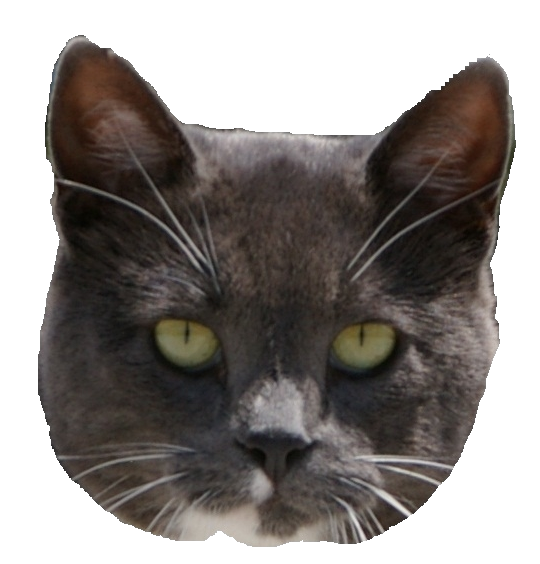
\includegraphics[width=1em]{leon.png}}
	\begin{document}
		\begin{itemize}
			\item[\meow] My cat's name is Leon
			\item[\meow] He is a handsome little man
			\item[\meow] Also a jerk
		\end{itemize}
	\end{document}
\end{filecontents*}

\compit{hiddenleonitemize}

\begin{filecontents*}{hiddenmicrotype.tex}
	\documentclass{article}
	\usepackage{lipsum}
	\usepackage{microtype}
	\usepackage[paperheight=5in,paperwidth=4in,margin=0.5in,heightrounded,showframe]{geometry}
	\begin{document}
		\lipsum[1]
	\end{document}
\end{filecontents*}

\compit{hiddenmicrotype}

\begin{filecontents*}{hiddentable.tex}
	\documentclass{article}
	\usepackage[table]{xcolor}
	\usepackage{multirow}
	\usepackage{hhline}
	\usepackage{graphicx}
	\newcolumntype{C}{>{\centering\arraybackslash}p{1cm}}
	
	\begin{document}
		\rowcolors{2}{gray!40}{gray!40}
		\renewcommand{\arraystretch}{1.1}
		\setlength{\arrayrulewidth}{0.6pt}
		\begin{tabular}{|C|>{\columncolor{gray!40}}C|*{5}{C|}}\hhline{*{7}{-}}
			\multicolumn{2}{|c|}{\cellcolor{gray!40}}& \multicolumn{5}{c|}{\cellcolor{white}Group III} \\\hhline{~~*{5}{-}}
			\multicolumn{2}{|c|}{III--V} & 5 & 13 & 31 & 69 & 81 \\
			\multicolumn{2}{|c|}{Compounds} & B & Al & Ga & In & Tl \\\hhline{*{7}{-}}
			\hiderowcolors
			&  7  & BN  & AlN    & GaN    & InN    & TlN \\
			&  N  &     &        & (3.4)  &        & \\\hhline{~*{6}{-}}
			&  15 & BP  & AlP    & GaP    & InP    & TlP \\
			&  P  &     & (2.55) & (2.24) & (1.27) & \\\hhline{~*{6}{-}}
			&  33 & BAs & AlAs   & GaAs   & InAs   & TlAs \\
			&  As &     &        & (1.35) &        & \\\hhline{~*{6}{-}}
			&  51 & BSb & AlSb   & GaSb   & InSb   & TlSb \\
			&  Sb &     &        & (9.67) &        & \\\hhline{~*{6}{-}}
			&  84 & BBi & AlBi   & GaBi   & InBi   & TlBi \\
			\multirow{-10}{*}{\rotatebox{90}{Group V}}
			&  Bi &     &        &        &        & \\\hhline{*{7}{-}}
			\multicolumn{4}{|p{\dimexpr4cm+6\tabcolsep+3\arrayrulewidth\relax}|}{\cellcolor{gray!40} Atomic number in black above element} &
			\multicolumn{3}{p{\dimexpr3cm+4\tabcolsep+2\arrayrulewidth\relax}|}{\cellcolor{gray!40} Energy band gap (eV) of some of the selected elements within bracket}\\\hhline{*{7}{-}}
		\end{tabular}
	\end{document}
\end{filecontents*}

\compit{hiddentable}

\begin{filecontents*}{hiddencitations.tex}
	\documentclass{article}
	\usepackage[paperheight=3in,paperwidth=3in,margin=0in]{geometry}
	\begin{document}
		Not only does the illustrious Dr. Honeycutt have a PhD in chemistry~\cite{dissertation}, but he likes to give technical talks~\cite{talk2014, talk2015}.  Other people even like giving presentations on his work~\cite{jacob2016}!
		\pagebreak
		\bibliographystyle{unsrt}
		\bibliography{bib}
	\end{document}
\end{filecontents*}

\immediate\write18{pdflatex hiddencitations.tex}
\immediate\write18{bibtex hiddencitations.aux}
\immediate\write18{pdflatex hiddencitations.tex}
\compit{hiddencitations}